\section{Các tính năng chính}
\subsection{Panels}
Grafana cung cấp các bảng biểu, đồ thị đa dạng bao gồm bản đồ nhiệt, histograms, đồ thị, biểu đồ địa lý để trực quan hoá dữ liệu một cách linh động theo bất kì cách nào chúng ta muốn.
\begin{figure}[H] % places figure environment here   
    \centering % Centers Graphic
    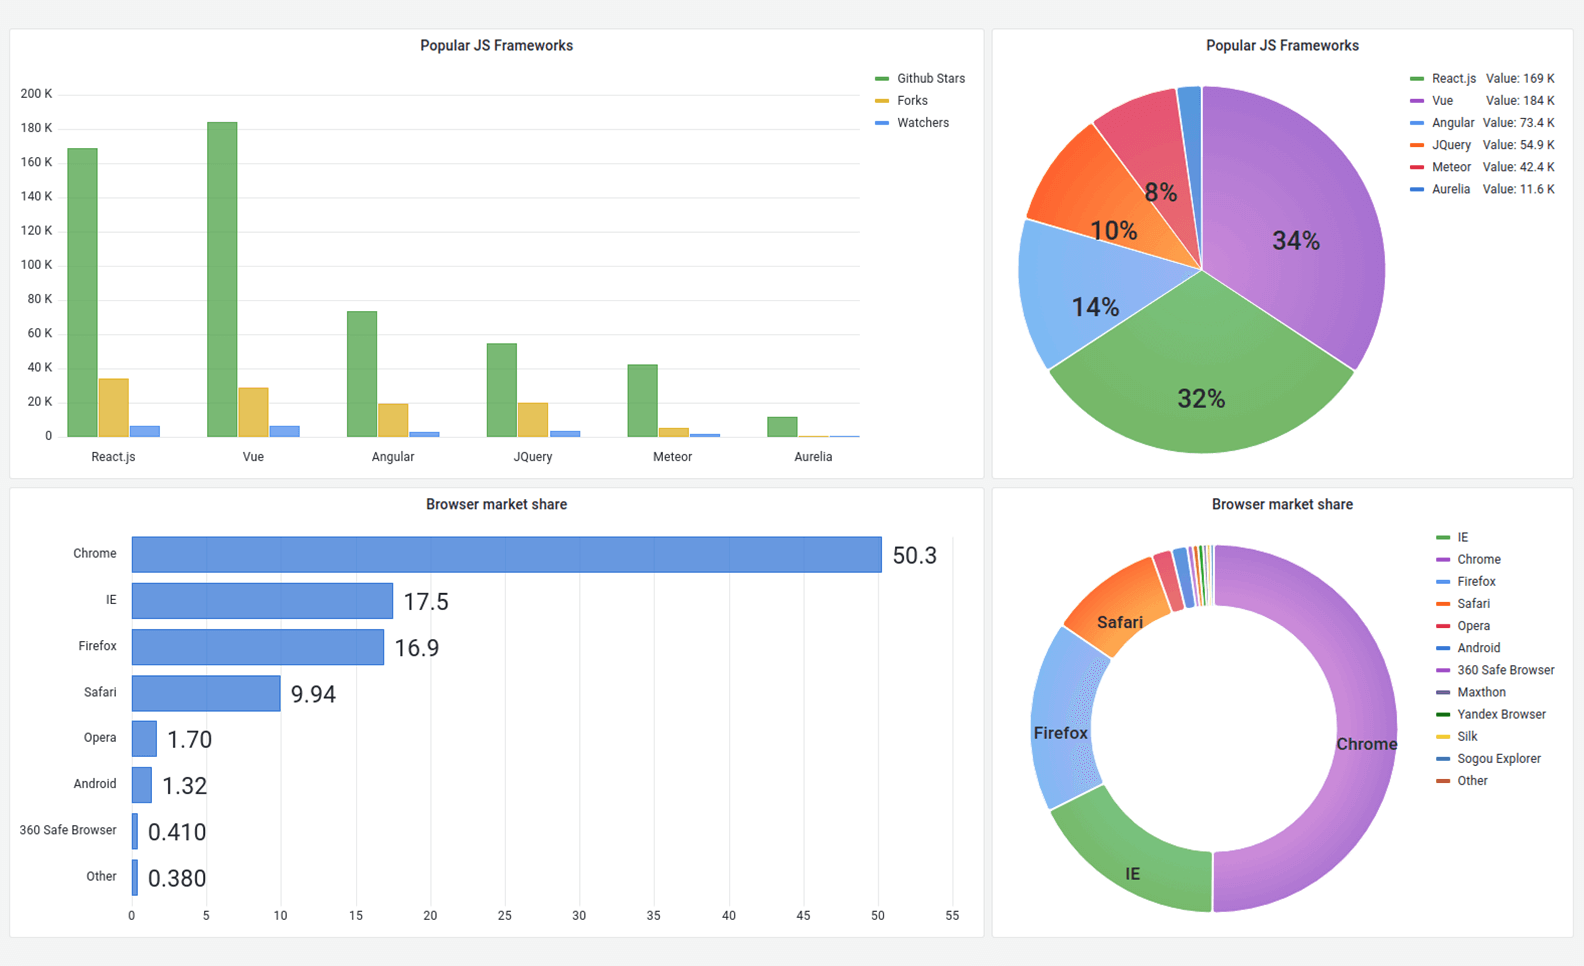
\includegraphics[width=0.8\textwidth]{figures/bar_chart_and_pie_chart_light_theme_sized.png} 
    \caption{Biểu đồ cột và biểu đồ tròn} % Creates caption underneath graph
    \label{fig:fig_01}
\end{figure}
\begin{figure}[H] % places figure environment here   
    \centering % Centers Graphic
    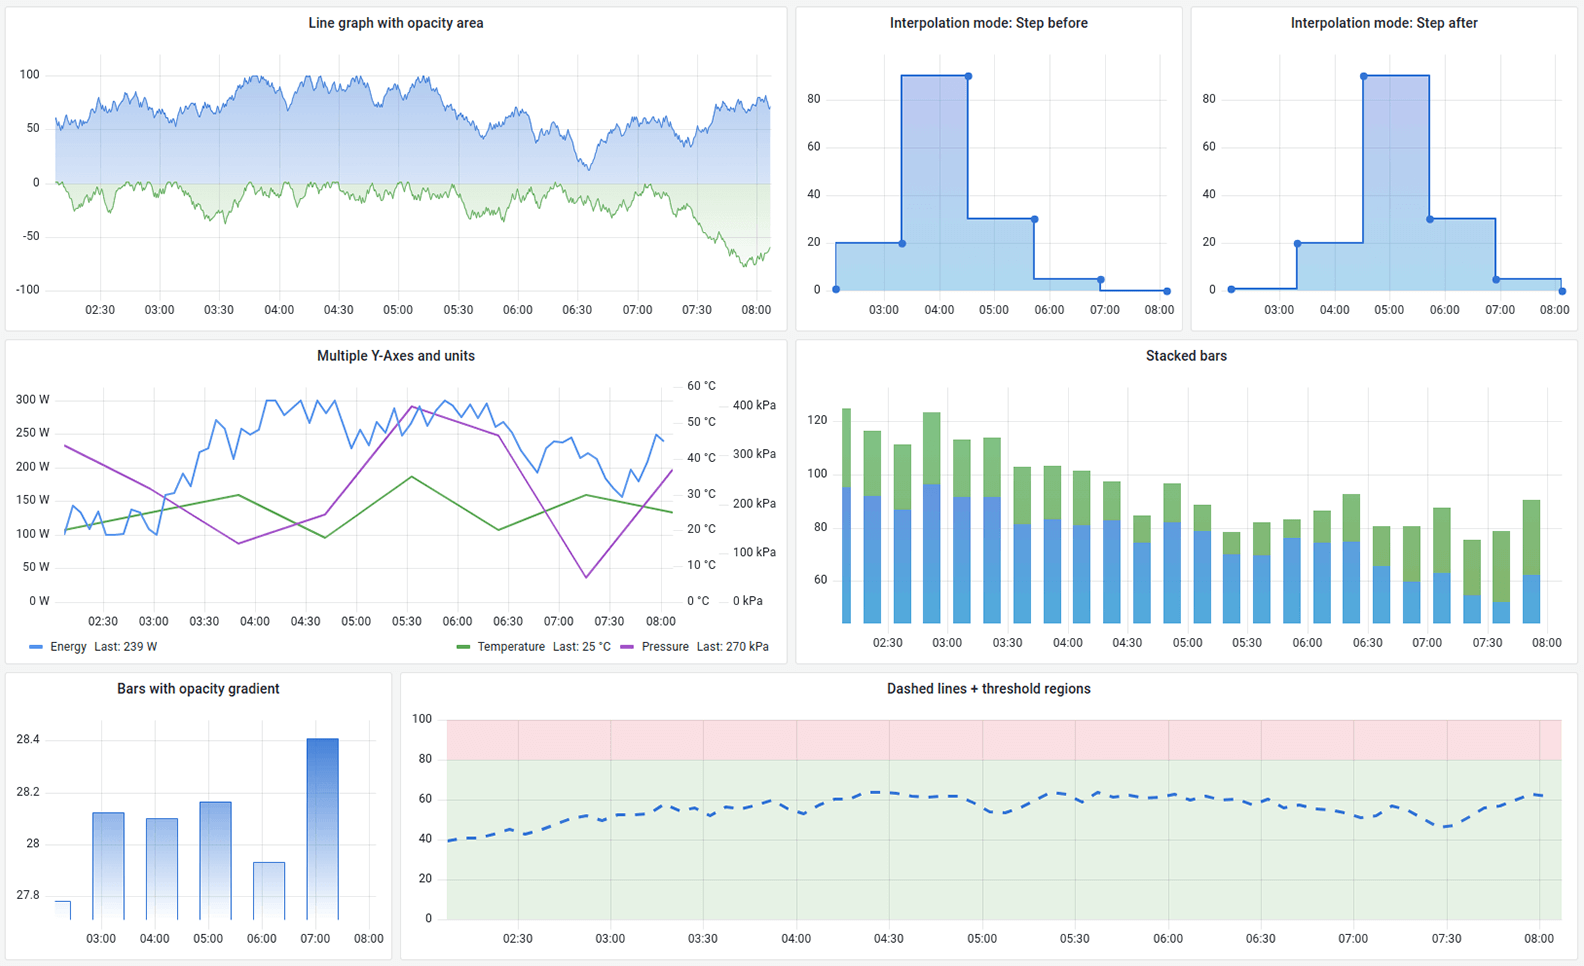
\includegraphics[width=0.8\textwidth]{figures/time_series_light_theme_sized.png} 
    \caption{Biểu đồ dữ liệu hướng thời gian} % Creates caption underneath graph
    \label{fig:fig_01}
\end{figure}
\begin{figure}[H] % places figure environment here   
    \centering % Centers Graphic
    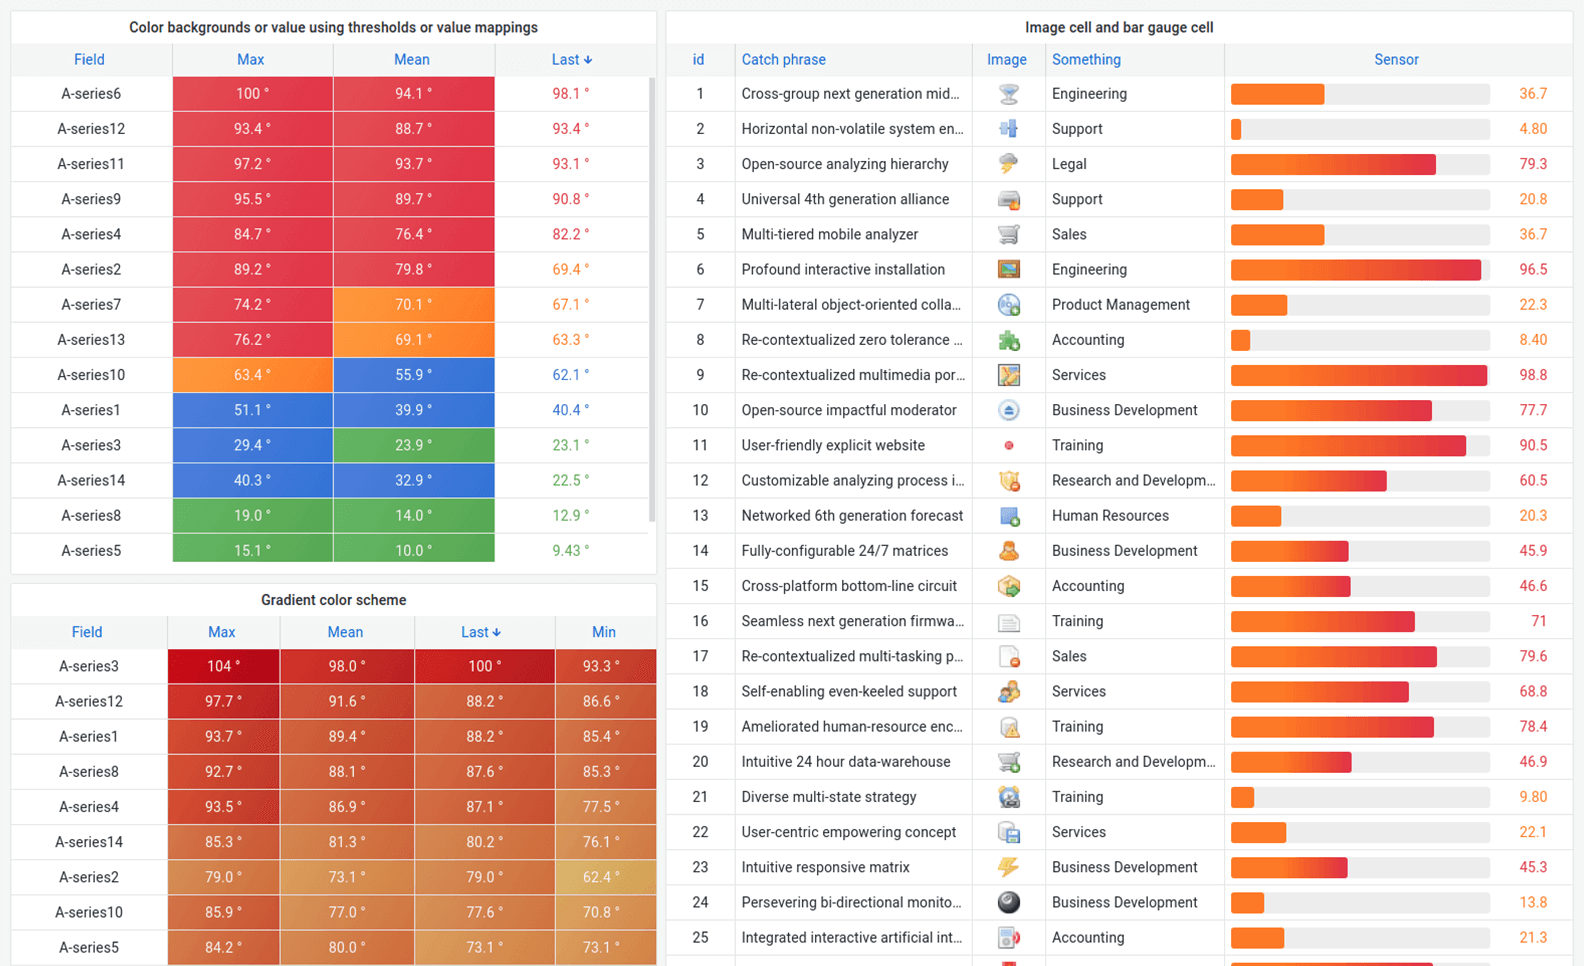
\includegraphics[width=0.8\textwidth]{figures/table_light_theme_sized.png} 
    \caption{Biểu dữ liệu dạng bảng} % Creates caption underneath graph
    \label{fig:fig_01}
\end{figure}
\begin{figure}[H] % places figure environment here   
    \centering % Centers Graphic
    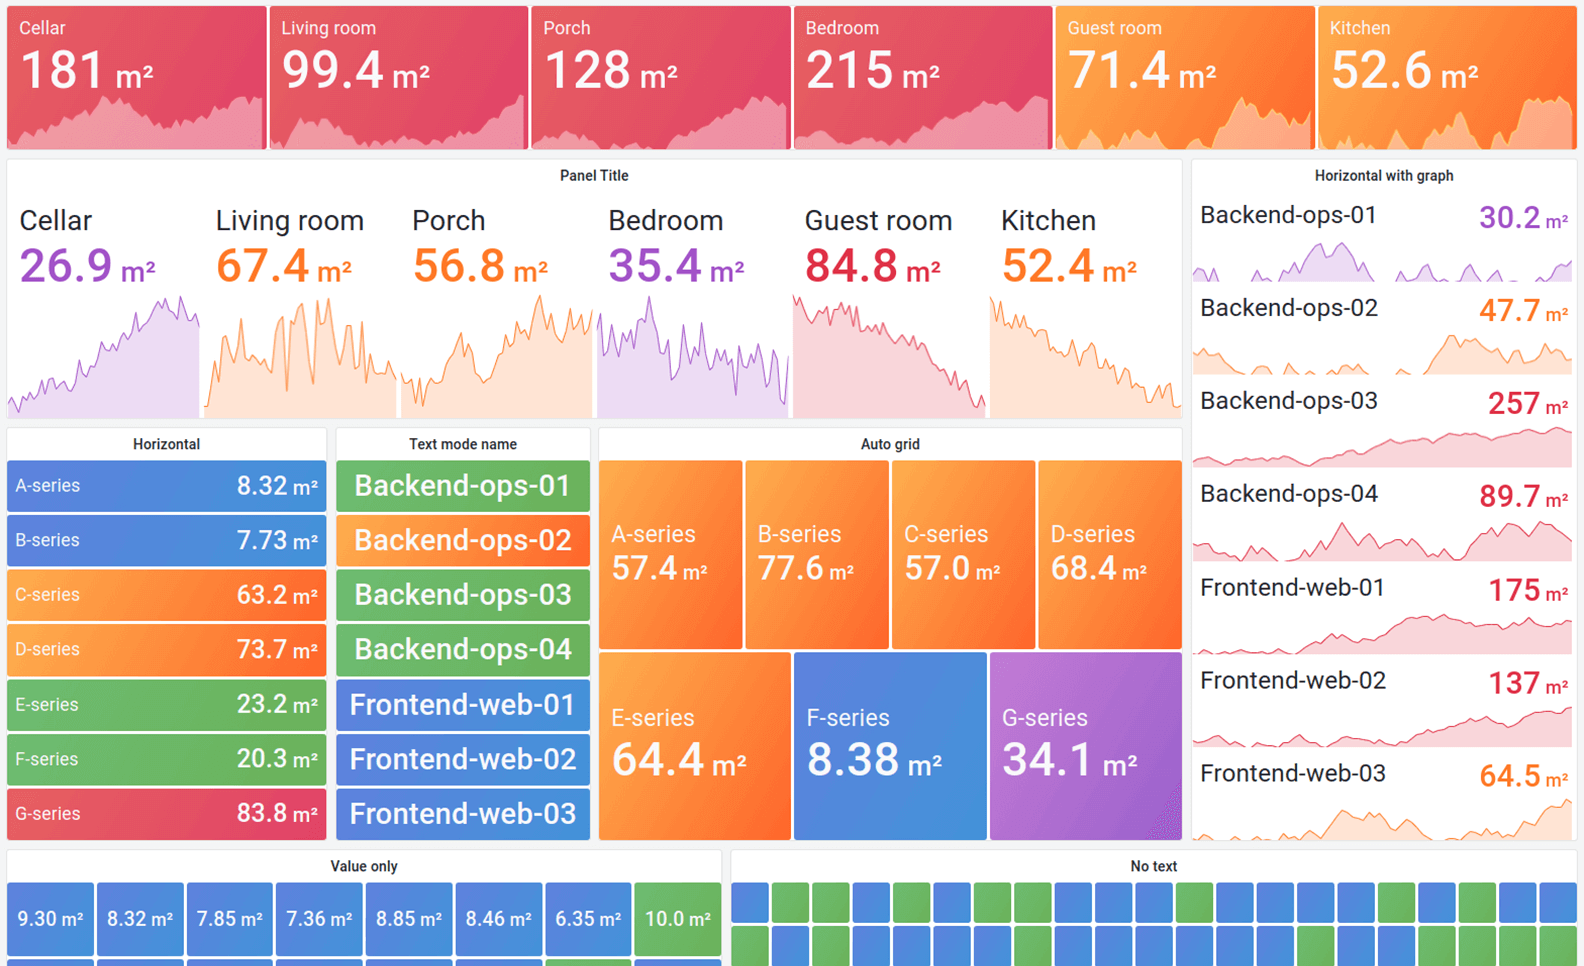
\includegraphics[width=0.8\textwidth]{figures/stat_light_theme_sized.png} 
    \caption{Biểu đồ thống kê} % Creates caption underneath graph
    \label{fig:fig_01}
\end{figure}

\subsection{Plugins}
\begin{figure}[H] % places figure environment here   
    \centering % Centers Graphic
    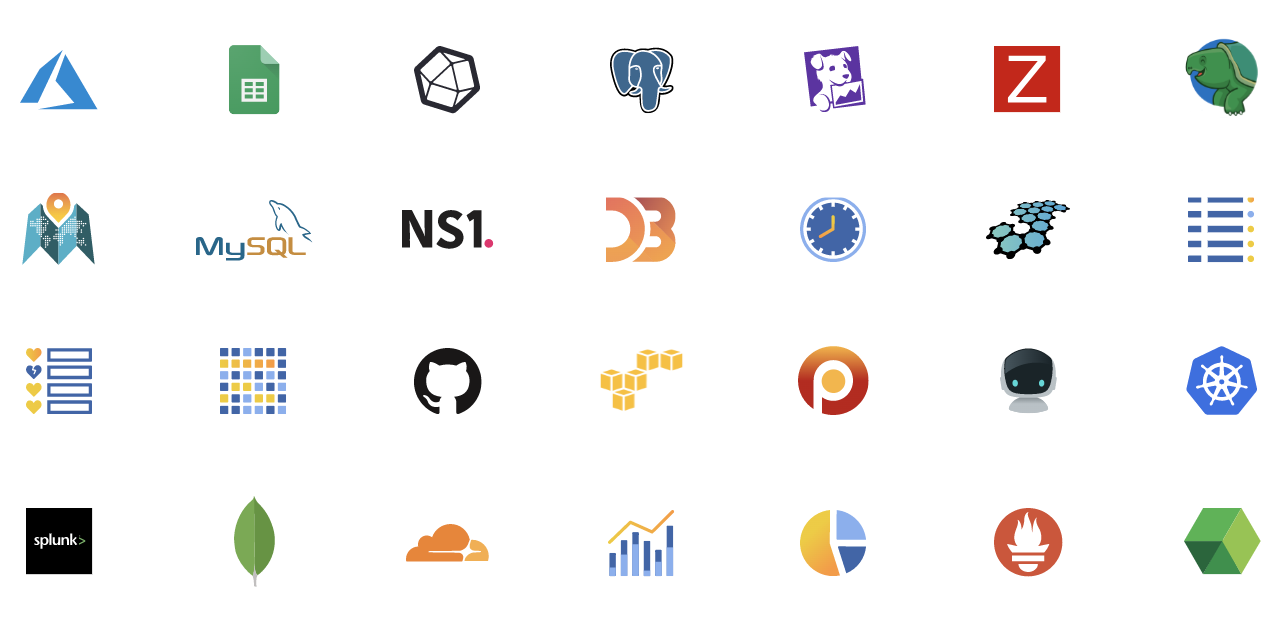
\includegraphics[width=0.8\textwidth]{figures/grafana_plugins.png} 
    \caption{Các tiện ích mở rộng} % Creates caption underneath graph
    \label{fig:fig_01}
\end{figure}
Grafna không yêu cầu phải lưu dữ liệu vào một cơ sở dữ liệu tập trung, thay vào đó nó cung cấp các tiện ích mở rộng cho phép ta kết nối tới nhiều loại cơ sở dữ liệu khách nhau. Ngoài ra Grafana cũng cho phép kết nối tới các công cụ nội bộ, cho phép doanh nghiệp triển khai một cách độc lập mà không cần phải thông qua một bên thứ 3 nữa. Ví dụ chúng ta có thể phân quyền người dùng với hệ thống xác thực tập trung riêng của doanh nghiệp hoặc cũng có thể tuỳ chỉnh hệ thống cảnh báo để gửi tin về hệ thống nhắn tin riêng mà không cần thông qua những hệ thống chung như email.